\subsection{Case 0, $M = N$}
ICA is applied on $\mathbf{Y}_s$ specified by $M\_ = 27$ and $L_s = 516$. 
The main algorithm is applied on $\mathbf{Y}_s$ without any reduction hence specified by $M = 27$ and $L_s = 516$, given $\hat{\mathbf{A}}_{\text{fix}}$ and $N = k$ provided from ICA.
Figure \ref{fig:M=N_1} show $\text{MSE}\left(\hat{\mathbf{X}}_{\text{main}},\hat{\mathbf{X}}_{\text{ICA}}\right)$ for all segments $s$. 
Figure \ref{fig:M=N_1_2} show the same plot but the y-axis is specified to the interval $[-10,50]$ for better visualization.
Furthermore, the MSE tolerance $= 5$ is plotted, indicting for each segment whether the estimate $\hat{\mathbf{X}}_{\text{main}}$ is sufficiency close to $\hat{\mathbf{X}}_{\text{main}}$. 
For a majority of the segments the MSE lies under the tolerance, but single outliers appears for which the MSE of the segment is significantly increased. Taking the average over all segments the average achieved MSE is $5.17$.    
\begin{figure}[H]
\begin{widepage}
    \begin{minipage}[t]{.45\textwidth}
		\centering
		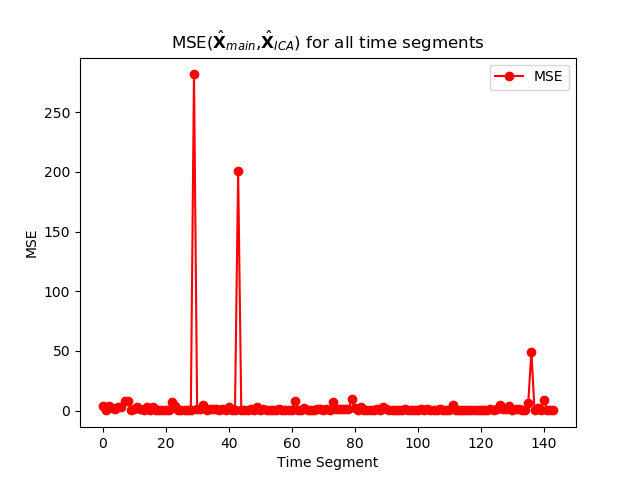
\includegraphics[width=1\linewidth]{figures/ch_7/resultat/average_mse_none_removed_ica}
	\caption{$\text{MSE} \left(\hat{\mathbf{X}}_{\text{main}}, \hat{\mathbf{X}}_{\text{ICA}}\right)$ for all $n_{\text{seg}} = $ 144 segments.}
	\label{fig:M=N_1}
    \end{minipage} 
    \hspace{0.5cm}
    \begin{minipage}[t]{.45\textwidth}
        \centering
		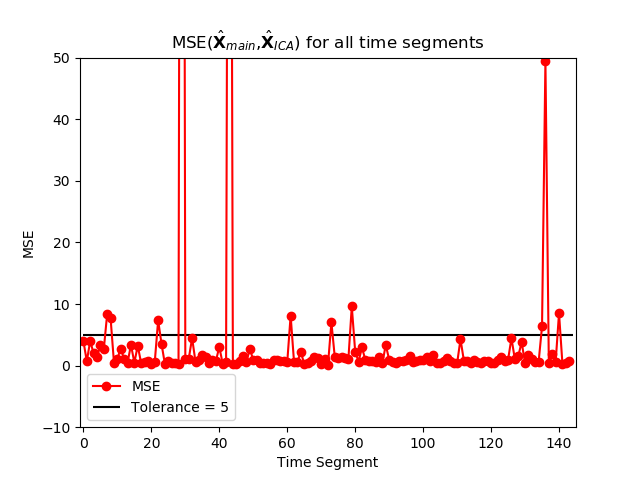
\includegraphics[width=1\linewidth]{figures/ch_7/resultat/average_mse_none_removed_ica_zoom.png}
	\caption{$\text{MSE} \left(\hat{\mathbf{X}}_{\text{main}}, \hat{\mathbf{X}}_{\text{ICA}}\right)$ for all $n_{\text{seg}} = $ 144 segments. Plotted only for the y-axis interval $[-10, 50]$ for better visualization.}
	\label{fig:M=N_1_2}
    \end{minipage}
\end{widepage}
\end{figure}
\noindent
To investigate the behavior of a single segment figure \ref{fig:M=N_2} show the MSE value computed for each row of the two estimates of a specific segment. 
That is MSE$(\hat{\mathbf{X}}_{\text{main}_{i}}$, $\hat{\mathbf{X}}_{\text{ICA}_{i}})$ for every row $i = 1, \dots, k$ in time segment $s = 5$. 
Additionally figure \ref{fig:M=N_3} show and compare the corresponding estimates for four random chosen sources. 
This allows for visual comparison of the estimates relative to the corresponding MSE value seen in figure \ref{fig:M=N_2}. 
Note that for better visual comparison each plotted row of $\hat{\mathbf{X}}_{\text{ICA}}$ is scaled with respect to the max value of the corresponding row in $\hat{\mathbf{X}}_{\text{main}}$.
From figure \ref{fig:M=N_2} it is seen that the estimate of each source result in a relative low MSE. This indicates that the main algorithm has managed to estimate the same source as the ICA algorithm. 
In contradiction to this, figure \ref{fig:M=N_3} do not confirm that the estimates are close, as generally the two signals in one plot does not follow the same trend.   
\begin{figure}[H]
\begin{widepage}
    \begin{minipage}[t]{.45\textwidth}
\centering
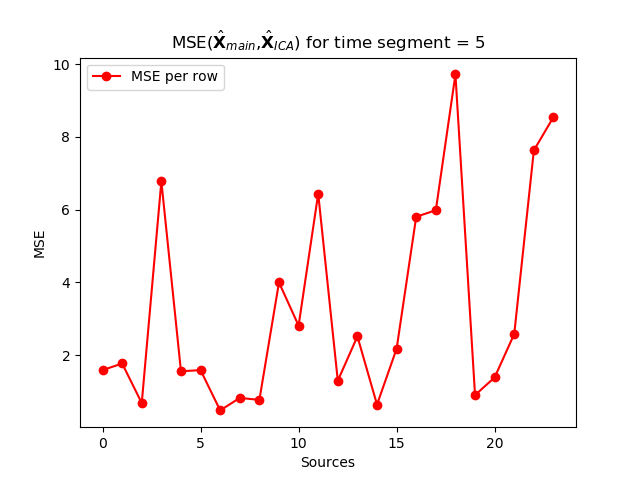
\includegraphics[width=1\linewidth]{figures/ch_7/resultat/mse_none_removed_ica_timeseg5.png}
\caption{MSE$\left(\hat{\mathbf{X}}_{\text{main}_{i}},\hat{\mathbf{X}}_{\text{ICA}_{i}}\right)$ for every row $i = 1, \dots, k$ in time segment $s=5$.}
\label{fig:M=N_2}
\end{minipage} 
\hspace{0.5cm}
\begin{minipage}[t]{.45\textwidth}
\centering
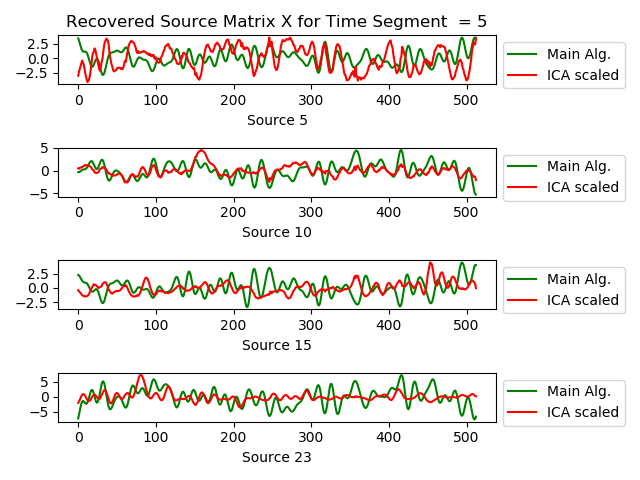
\includegraphics[width=1\linewidth]{figures/ch_7/resultat/EEG_none_removed_scaled_timeseg5S1_CClean.png}
\caption{Plot comparing four random chosen rows from $\hat{\mathbf{X}}_{\text{main}}$ and $\hat{\mathbf{X}}_{\text{ICA}}$ from time segment $s = 5$ with $M = N$ and $k=23$. Note $\hat{\mathbf{X}}_{\text{ICA}}$ is scaled for better visualization.}
	\label{fig:M=N_3}
    \end{minipage}
\end{widepage}
\end{figure}
\noindent
The test is repeated for every data set, and the results are summarized in table \ref{tab:case_0}. 
In general a low MSE is achieved in average over all segments of one data set relative to the tolerance.
And the corresponding percentage is likewise relative high, with an average at $83\%$. 
A single result is seen to deviate from the tendency, which is the data set of test subject 3 with closed eyes. 
Here a significant high average MSE value is found, indicating a majority of the segment has resulted in a significantly high MSE, while a percentage of $63\%$ was below the tolerance. 
In chapter \ref{ch:implementation} it is found that the main algorithm was capable of providing an almost exact estimate for $M = N$ when the true $\mathbf{A}$ is provided. 
Thus, it is expected that the general performance is decreased in this case where the true $\mathbf{A}$ is unknown and $\hat{\mathbf{A}}_{\text{fix}}$ is given.

The achieved results will serve as reference when analyzing the results of the following cases where the main algorithm is applied on data set with reduced number of sensors compared to the original data set.         
\begin{table}[H]
\centering
\begin{tabular}{|c|c|c|c|c|c|c|}
\hline
\multirow{2}{*}{\textbf{\begin{tabular}[c]{@{}c@{}}Case 0 \\ $M = N$\end{tabular}}} & \multicolumn{2}{c|}{Test subject 1} & \multicolumn{2}{c|}{Test subject 2} & \multicolumn{2}{c|}{Test subject 3} \\ \cline{2-7} 
                                                                                  & Open             & Close            & Open             & Close            & Open            & Close             \\ \hline
\multicolumn{1}{|c|}{Average MSE()}                                               & 2.913            & 5.172            & 1.572            & 15.06            & 4.753            & 19.44           \\ \hline
\begin{tabular}[c]{@{}c@{}}Segments below \\ tolerance in \%\end{tabular}          & 91             & 92            & 98 & 61             & 87            & 63 \\ \hline
\end{tabular}
\caption{Summarized results for case 0. Test is performed on the every data set.}
\label{tab:case_0}
\end{table}	
\noindent

\subsection{Case 1, $M < N$}
The main algorithm is applied on $\mathbf{Y}_s$, where the number of sensors is reduced by one-third. 
As such the main algorithm is applied on $\mathbf{Y}_s$ specified by $M = 18$ and $L_s = 516$, given $\hat{\mathbf{A}}_{\text{fix}}$ and $N = k$ provided from ICA. 
ICA is applied on the original data set with segments $\mathbf{Y}_s$ specified by $M\_ = 27$ and $L_s = 516$.  
The viewed plots correspond to those of case 0, but for the reduced number of sources $M < N$, hence detailed plot description is omitted here.   

From figure \ref{fig:M<N_1} and \ref{fig:M<N_1_2} it is seen that a majority of the segments have MSE value close to the tolerance, but the number of outliers have increased compared to case 0.
This indicates that for an increased number of segments the main algorithm do not manage to estimate enough sources sufficiently in order to stay below the tolerance. Taking the average over all segments the average achieved MSE is $5.35$.
\begin{figure}[H]
\begin{widepage}
    \begin{minipage}[t]{.45\textwidth}
		\centering
		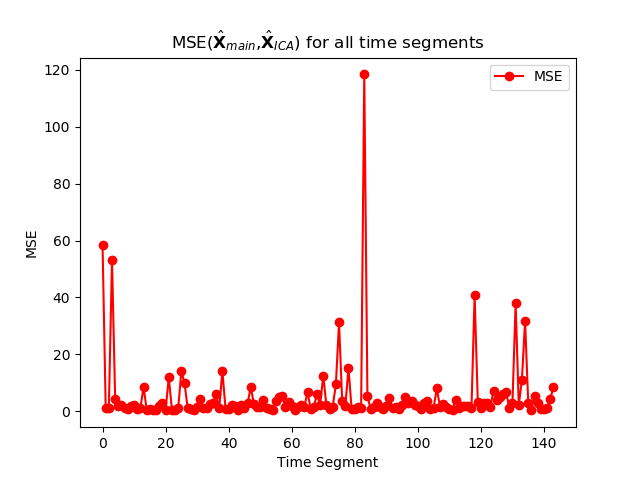
\includegraphics[width=1\linewidth]{figures/ch_7/resultat/average_mse_third_removed_ica}
	\caption{MSE$\left(\hat{\mathbf{X}}_{\text{main}},\hat{\mathbf{X}}_{\text{ICA}}\right)$ for all $n_{\text{seg}} = $ 144 segments.}
	\label{fig:M<N_1}
    \end{minipage} 
\hspace{0.5cm}
    \begin{minipage}[t]{.45\textwidth}
        \centering
		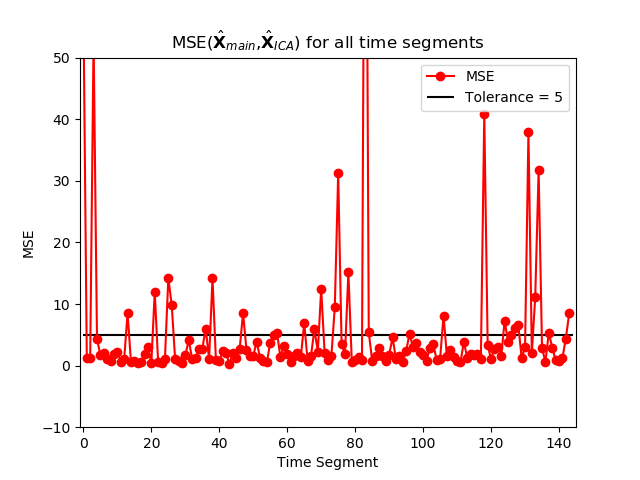
\includegraphics[width=1\linewidth]{figures/ch_7/resultat/average_mse_third_removed_ica_zoom.png}
	\caption{MSE$\left(\hat{\mathbf{X}}_{\text{main}},\hat{\mathbf{X}}_{\text{ICA}}\right)$ for all $n_{\text{seg}} = $ 144 segments. Plotted only for the y-axis interval $[-10, 50]$ for better visualization.}
	\label{fig:M<N_1_2}
    \end{minipage}
\end{widepage}
\end{figure}
\noindent 
From figure \ref{fig:M<N_2} and \ref{fig:M<N_3} showing the results of segment 5, it is seen that the MSE for each source has increased slightly compared to case 0. 
This supports the observation from figure \ref{fig:M<N_1_2}.      
\begin{figure}[H]
\begin{widepage}
    \begin{minipage}[t]{.45\textwidth}
\centering
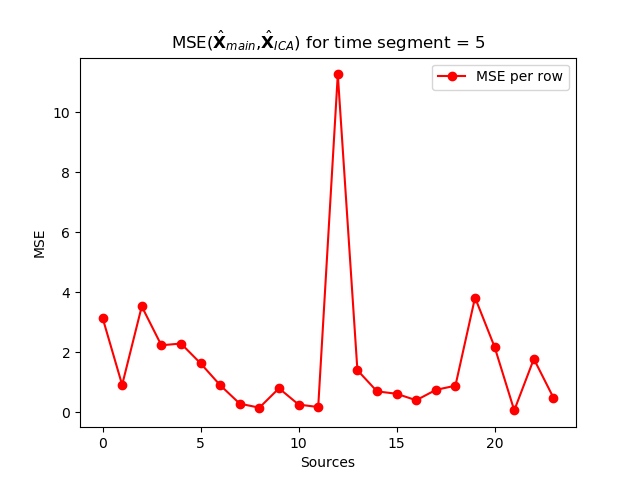
\includegraphics[width=1\linewidth]{figures/ch_7/resultat/mse_third_removed_ica_timeseg5.png}
\caption{MSE$\left(\hat{\mathbf{X}}_{\text{main}_{i}},\hat{\mathbf{X}}_{\text{ICA}_{i}}\right)$ for every row $i = 1, \dots, k$ in time segment $s=5$.}
\label{fig:M<N_2}
\end{minipage} 
\hspace{0.5cm}
\begin{minipage}[t]{.45\textwidth}
\centering
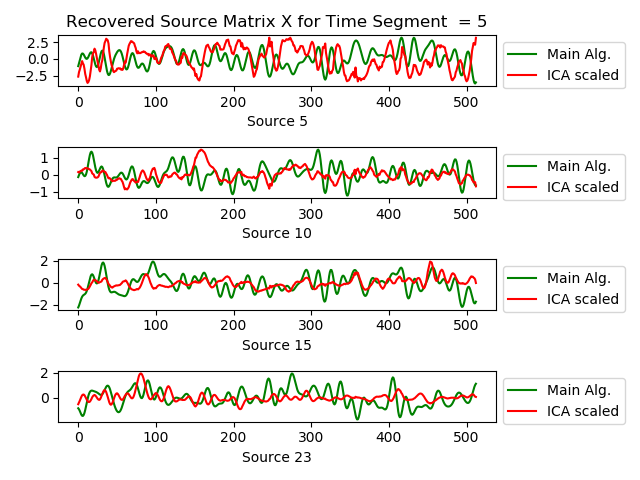
\includegraphics[width=1\linewidth]{figures/ch_7/resultat/EEG_third_removed_scaled_timeseg5S1_CClean.png}
\caption{Plot comparing four random chosen rows from $\hat{\mathbf{X}}_{\text{main}}$ and $\hat{\mathbf{X}}_{\text{ICA}}$ from time segment $s = 5$ with $M = N$ and $k=23$. Note $\hat{\mathbf{X}}_{\text{ICA}}$ is scaled for better visualization.}
	\label{fig:M<N_3}
    \end{minipage}
\end{widepage}
\end{figure}
\noindent
The test is repeated for every data set, and the results are summarized in table \ref{tab:case_1}. 
Comparing table \ref{tab:case_1} to table \ref{tab:case_0}, it is seen that the percentage of segments below the tolerance are decreasing, with the majority being close to $50\%$.
This is roughly indicating that half of the time the main algorithm do not manage to provide a sufficient estimate when $M = 2/3N$.  
Furthermore, both the average MSE and the corresponding percentages appear fluctuating relative to case 0 indicating some unreliability in the results.  
\begin{table}[H]
\centering
\begin{tabular}{|c|c|c|c|c|c|c|}
\hline
\multirow{2}{*}{\textbf{\begin{tabular}[c]{@{}c@{}}Case 1 \\ $M < N$\end{tabular}}} & \multicolumn{2}{c|}{Test subject 1} & \multicolumn{2}{c|}{Test subject 2} & \multicolumn{2}{c|}{Test subject 3} \\ \cline{2-7} 
                                                                                  & Open             & Close            & Open             & Close            & Open              & Close           \\ \hline
\multicolumn{1}{|c|}{Average MSE()}                                               & 9.79            & 5.351            & 13.89            & 15.13            & 6.25          & 18.21          \\ \hline
\begin{tabular}[c]{@{}c@{}}Segments below \\ tolerance in \%\end{tabular}          & 53             & 80             & 66 & 46             & 77              & 48            \\ \hline
\end{tabular}
\caption{Summarized results for case 1. Test is performed on the every data set.}
\label{tab:case_1}
\end{table}
\noindent

\subsection{Case 2, $M << N$}
The main algorithm is applied on $\mathbf{Y}_s$, where the number of sensors is reduced to half. 
As such the main algorithm is applied on $\mathbf{Y}_s$ specified by $M = 13$ and $L_s = 516$, given $\hat{\mathbf{A}}_{\text{fix}}$ and $N = k$ provided from ICA.  
ICA is applied on the original data set with segments $\mathbf{Y}_s$ specified by $M\_= 27$ and $L_s = 516$. 
The viewed plots correspond to those of case 0 and case 1, but for further reduce number of sources $M << N$, hence detailed plot description is omitted.   

From figure \ref{fig:M<<N_1} and \ref{fig:M<<N_1_2} it is seen that the MSE value for each segment is more widely scatted around the tolerance, compared to case 0 and 1. 
Outliers, where the MSE value has increased significantly, do also occur similar to case 1. 
This indicates that the performance of the main algorithm has decreased further, compared to case 1. Taking the average over all segments the average achieved MSE is $11.36$.
\begin{figure}[H]
\begin{widepage}
    \begin{minipage}[t]{.45\textwidth}
		\centering
		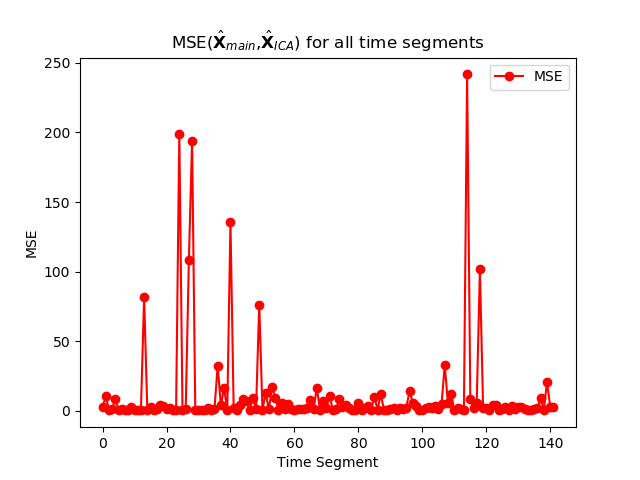
\includegraphics[width=1\linewidth]{figures/ch_7/resultat/average_mse_second_removed_ica}
	\caption{MSE$\left(\hat{\mathbf{X}}_{\text{main}},\hat{\mathbf{X}}_{\text{ICA}}\right)$ for all $n_{\text{seg}} = $ 144 segments.}
	\label{fig:M<<N_1}
    \end{minipage} 
\hspace{0.5cm}
    \begin{minipage}[t]{.45\textwidth}
        \centering
		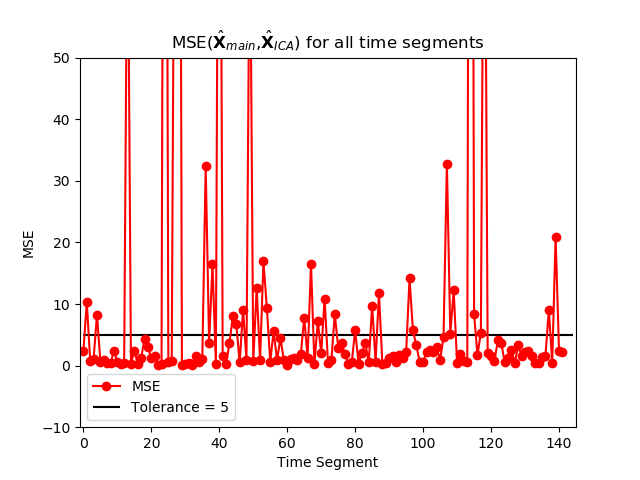
\includegraphics[width=1\linewidth]{figures/ch_7/resultat/average_mse_second_removed_ica_zoom.png}
	\caption{MSE$\left(\hat{\mathbf{X}}_{\text{main}},\hat{\mathbf{X}}_{\text{ICA}}\right)$ for all $n_{\text{seg}} = $ 144 segments. Plotted only for the y-axis interval $[-10, 50]$ for better visualization.}
	\label{fig:M<<N_1_2}
    \end{minipage}
\end{widepage}
\end{figure}
\noindent 
The above indication is supported by figure \ref{fig:M<<N_2} and \ref{fig:M<<N_3} showing an general increase in MSE. 
However, segment 5 makes a fairly good example as the majority of the sources have achieves a MSE below the tolerance of 5. 
From figure \ref{fig:M<<N_3} the increased MSE do not appear visually compared to either case 1 or case 0.        
\begin{figure}[H]
\begin{widepage}
    \begin{minipage}[t]{.49\textwidth}
\centering
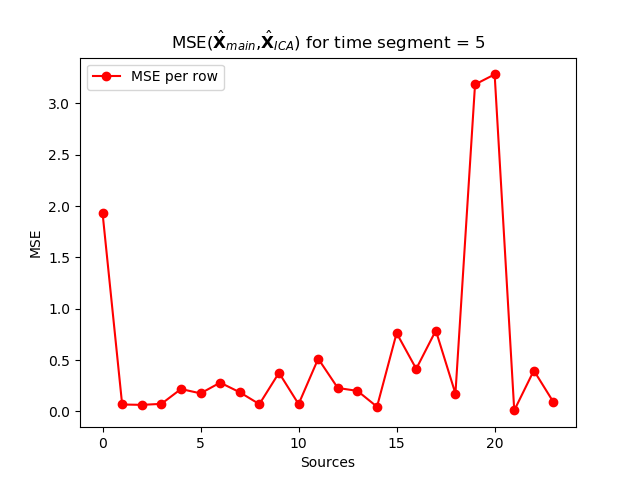
\includegraphics[width=1\linewidth]{figures/ch_7/resultat/mse_second_removed_ica_timeseg5.png}
\caption{MSE$\left(\hat{\mathbf{X}}_{\text{main}_{i}},\hat{\mathbf{X}}_{\text{ICA}_{i}}\right)$ for every row $i = 1, \dots, k$ in time segment $s = 5$.}
\label{fig:M<<N_2}
\end{minipage} 
\hspace{.5cm}
\begin{minipage}[t]{.49\textwidth}
\centering
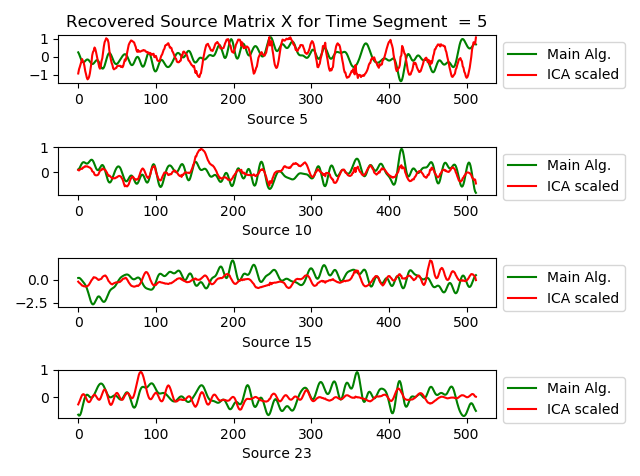
\includegraphics[width=1\linewidth]{figures/ch_7/resultat/EEG_second_removed_scaled_timeseg5S1_CClean.png}
\caption{Plot comparing four random chosen rows from $\hat{\mathbf{X}}_{\text{main}}$ and $\hat{\mathbf{X}}_{\text{ICA}}$ from time segment $s = 5$ with $M << N$ and $k=23$. Note $\hat{\mathbf{X}}_{\text{ICA}}$ is scaled for better visualization.}
	\label{fig:M<<N_3}
    \end{minipage}
\end{widepage}
\end{figure}
\noindent
The test is repeated for every data set, and the results are summarized in table \ref{tab:case_2}. Comparing table \ref{tab:case_0} to table \ref{tab:case_1} it is generally seen that the percentage of segments below the tolerance are not decreased but improved.
Though, without getting close to the tendency from case 0. 
Furthermore, the average MSE have not increased remarkably compared to case 1. 
As such the performance of the main algorithm in case 2 is in general not found to be worse than for case 1.
However, a clear improvement is not seen either.  
\begin{table}[H]
\centering
\begin{tabular}{|c|c|c|c|c|c|c|}
\hline
\multirow{2}{*}{\textbf{\begin{tabular}[c]{@{}c@{}}Case 2\\ $M << N$\end{tabular}}} & \multicolumn{2}{c|}{Test subject 1} & \multicolumn{2}{c|}{Test subject 2} & \multicolumn{2}{c|}{Test subject 3} \\ \cline{2-7} 
                                                                                  & Open             & Close            & Open             & Close            & Open             & Close            \\ \hline
\multicolumn{1}{|c|}{Average MSE()}                                               & 8.378            & 11.36            & 19.58            & 13.11            & 13.99           & 11.96            \\ \hline
\begin{tabular}[c]{@{}c@{}}Segments below \\ tolerance in \%\end{tabular}          & 75             & 74             & 42 & 72             & 69             & 69 \\ \hline
\end{tabular}
\caption{Summarized results for case 2. Test is performed on the every data set.}
\label{tab:case_2}
\end{table}
\noindent
